\documentclass{article}

\usepackage{graphicx}
\usepackage{subfig}
\usepackage{amsmath}
%\usepackage{amsmath,rotating}

\title{Laminar, Three-dimensional Open Jet}

\date{}

\begin{document}

\maketitle

\section{Introduction}
This case provides a description for three-dimensional laminar
open jet flow (bottom constrained plane) with constant properties. A passive
scale mixture fraction is activated; inflow velocity is a constant value
absent of any profile.

\section{Theory}
The three-dimensional geometry for this tutorial is captured in 
Figure~\ref{fig:geom}. Here, the cylindrical domain is defined by the 
vertical height, $H$, the outer diameter, $D_o$, and inlet pipe diameter $d_o$ and 
specified to be 50 cm, 15 cm, and 1.0 cm, respectively. 

The bottom plane contains an inflow and bottom wall while the side and top are represented
as an open boundary condition where static pressure is specified.

\begin{figure}[!htbp]
  \centering
  {
   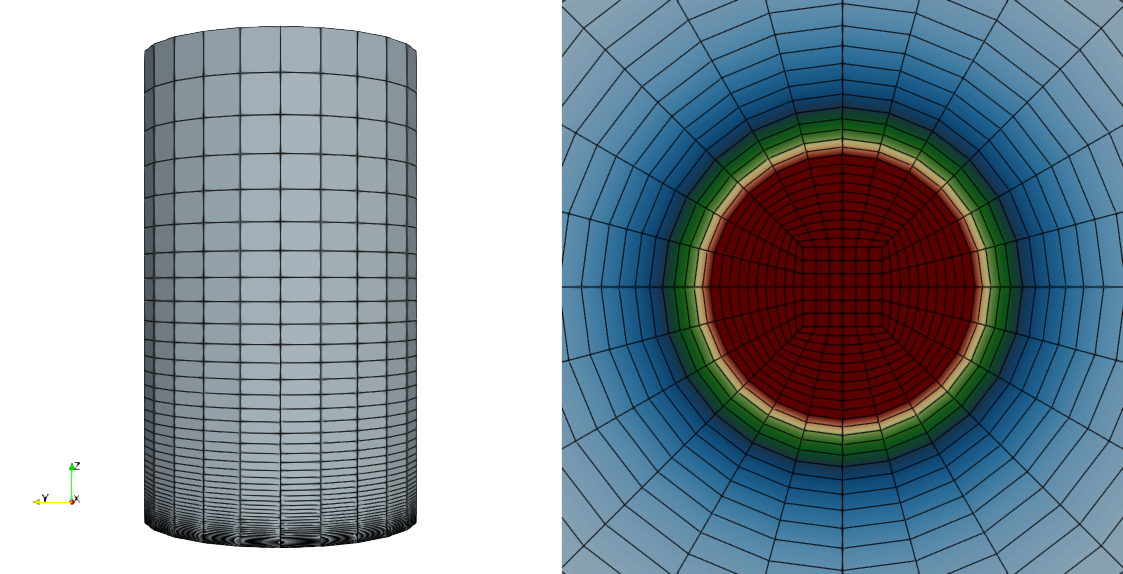
\includegraphics[height=2.0in]{images/3d_hex8_open_jet_geom.png}
  }
  \caption{Three-dimensional open jet flow configuration. Shadings on the
right side of the figure are for mixture fraction, $Z$.}
  \label{fig:geom}
\end{figure}

The variable-density low-Mach equation set is defined by the continuity and momentum equation,

\begin{align}
  \frac {\partial \rho }{\partial t} + \frac{ \partial \rho u_j}{\partial x_j} = 0.
\label{eq:contEq}
\end{align} 

\begin{align}
  \frac {\partial \rho u_i }{\partial t} + \frac{ \partial \rho u_j u_i}{\partial x_j} 
-\frac{\partial \sigma_{ij}}{\partial x_j} = 0.
\label{eq:momEq}
\end{align}
%
In the above equation, $\rho$ is the fluid density and $u_j$ is the fluid velocity. 
The stress tensor is provided by
\begin{align}
\sigma_{ij}  = 2 \mu S^*_{ij} - P \delta_{ij},
\end{align}
%
where the traceless rate-of-strain tensor is defined as
\begin{align}
S^*_{ij}  = S_{ij} - \frac{1}{3} \delta_{ij} S_{kk} \nonumber
		     = S_{ij} - \frac{1}{3} \frac{\partial  u_k }{\partial x_k}\delta_{ij}.
\end{align}
In a low-Mach flow, the above pressure, $P$, is the perturbation about the thermodynamic
pressure, $P^{th}$. 

For the open jet configuration of interest, a passive scalar transport equation for mixture 
fraction is activated and defined as the mass fraction of species that originates 
from the inlet boundary condition,

\begin{align}
  \frac {\partial \rho Z }{\partial t} + \frac{ \partial \rho u_j Z}{\partial x_j} 
+\frac{\partial q_j }{\partial x_j} = 0,
\label{eq:zEq}
\end{align}
where the diffusive flux vector is given by $q_j = \frac{\mu}{Sc}\frac{\partial Z}{\partial x_j}$.
Here, the Schmidt number is given as a function of density and mass diffusivity $D$, as
$Sc = \frac{\mu}{\rho D}$. 

It is noted that although the domain is cylindrical and axisymmetric in nature, we present
the equation set in a Cartesian coordinate system.

\subsection{Analytical Profiles}
Similarity approximations are available for the three-dimensional open jet configuration.

\section{Results}
Let us test a simulation in which the Reynolds number based on inlet diameter and 
inlet velocity comprised of air is 100. By constraining the Reynolds number, density, viscosity,
and inlet pipe diameter, the inflow velocity ($u_{inlet}$) in the z-direction is obtained via,

\begin{align}
  u_{inlet} = \frac{\mu Re}{\rho d_o}.
\label{eq:muForm}
\end{align}
%
Values for density, viscosity, and inflow velocity are 1.0e-3 $g/cm^3$, 2.0e-4 $dyne-s/cm^3$, 
20 $cm/s$, respectively.
\subsection{Simulation Specification and Results}

For the $Re = 100$ configuration, the simulation is run using a Hex8 (linear hexahedral)
mesh. In Figure~\ref{fig:results}, mixture fraction and magnitude of velocity shadings 
are provided for the specifications provided above.

\begin{figure}[!htbp]
 \subfloat[]
  \centering
  {
   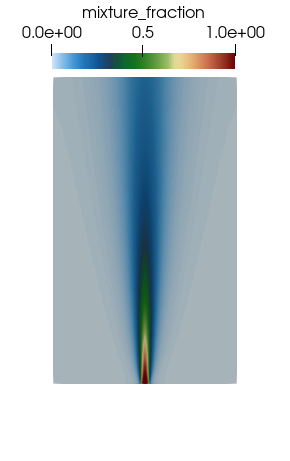
\includegraphics[height=3.0in]{images/3d_hex8_open_jet_mix_frac.png}
  }
  \subfloat[]
  \centering
  {
   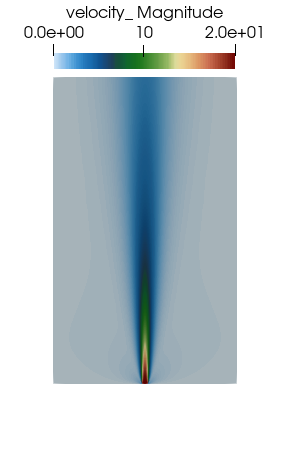
\includegraphics[height=3.0in]{images/3d_hex8_open_jet_umag.png}
  }
  \caption{Planar mixture fraction (a) and velocity magnitude (b) shadings for the $Re = 100$ jet case.}
  \label{fig:results}
\end{figure}

In Figure~\ref{fig:centerline}, the centerline normalized mixture fraction and vertical velocity
are presented.
%
\begin{figure}[!htbp]
  \centering
  {
   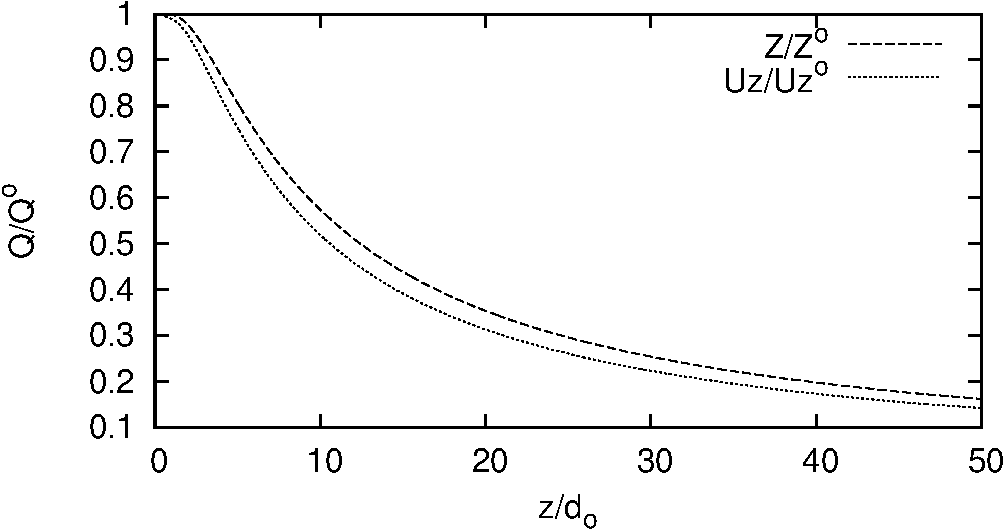
\includegraphics[height=2.0in]{images/CenterlineData-crop.pdf}
  }
  \caption{Normalized velocity and normalized-mixture fraction centerline plot for the $Re = 100$ jet case.}
  \label{fig:centerline}
\end{figure}
%
Finally, to illustrate the self-similar radial profiles for the downstream locations ($\frac{z}{d_o}$ of 5, 10,
and 20), see Figure~\ref{fig:similar}. For this procedure, the maximum velocity that occurs on the centerline
is captured at each downstream location. The radial half length, $r_h$, is defined as the radial position where the
velocity is one-half the peak value on the centerline. The self-similar jet profile is strongly correlated past 
$\frac{z}{d_o}$ of five - well beyond the core collapse of the jet.

\begin{figure}[!htbp]
  \centering
  {
   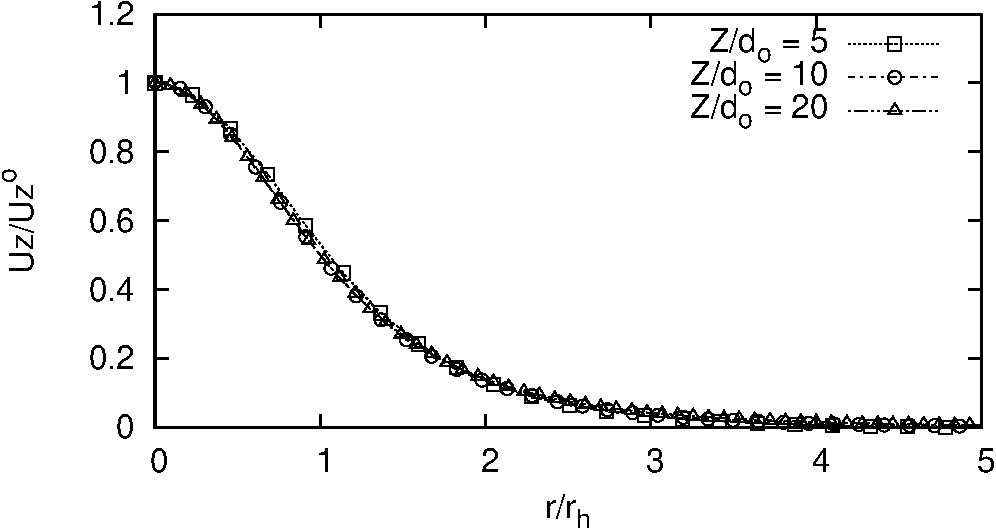
\includegraphics[height=2.0in]{images/ZdHalf-crop.pdf}
  }
  \caption{Normalized vertical velocity as a function of normalized radial distance (by radial half distance, 
$r_h$) for the $Re = 100$ jet case.}
  \label{fig:similar}
\end{figure}

\section{Discussion Points}

There are several interesting activities associated with this sample case including
the following:

\begin{itemize}
	\item Ensure that the underlying model suite is well understood.
	\item Explore the mesh and input file associated with this case.
	\item Explore the removal of the bottom wall plane in favor of an open boudnary condition with 
          and without total pressure specification.
        \item Comment on the resulting core collapse distance and the self-similar behavior.
\end{itemize}

\end{document}
